\documentclass{article}
\PassOptionsToPackage{numbers,compress}{natbib}
\usepackage[final]{template22}
\usepackage{indentfirst}
\setlength{\parindent}{2em}
% Common packages
\usepackage[utf8]{inputenc} % allow utf-8 input
\usepackage[T1]{fontenc}    % use 8-bit T1 fonts
\usepackage{microtype}
\usepackage{times}
\usepackage{graphicx}
\usepackage{amsmath,amssymb,mathbbol}
% \usepackage{algorithmic}
% \usepackage[linesnumbered,ruled,vlined]{algorithm2e}
\usepackage{acronym}
\usepackage{enumitem}
\usepackage[pagebackref=true,breaklinks=true,colorlinks]{hyperref}
\usepackage{balance}
\usepackage{xspace}
\usepackage{setspace}
\usepackage[skip=3pt,font=small]{subcaption}
\usepackage[skip=3pt,font=small]{caption}
\usepackage[dvipsnames]{xcolor}
\usepackage[capitalise]{cleveref}
\usepackage{booktabs,tabularx,colortbl,multirow,array,makecell}
% \usepackage{overpic,wrapfig}

\usepackage{fancyhdr}
\hypersetup{pdfencoding=auto,colorlinks=true,allcolors=black}
\renewcommand{\headrulewidth}{0.5pt}
\renewcommand{\footrulewidth}{0pt}
\fancyhf{}
\fancyhead[C]{}
\fancyhead[C]{}
\fancyfoot[C]{\thepage}

% Handy shorthand
\makeatletter
\DeclareRobustCommand\onedot{\futurelet\@let@token\@onedot}
\def\@onedot{\ifx\@let@token.\else.\null\fi\xspace}
\def\eg{\emph{e.g}\onedot} 
\def\Eg{\emph{E.g}\onedot}
\def\ie{\emph{i.e}\onedot} 
\def\Ie{\emph{I.e}\onedot}
\def\cf{\emph{c.f}\onedot} 
\def\Cf{\emph{C.f}\onedot}
\def\etc{\emph{etc}\onedot} 
\def\vs{\emph{vs}\onedot}
\def\wrt{w.r.t\onedot} 
\def\dof{d.o.f\onedot}
\def\etal{\emph{et al}\onedot}
\makeatother

\definecolor{gray}{gray}{0.9}

% Handy math ops
\DeclareMathOperator*{\argmax}{arg\,max}
\DeclareMathOperator*{\argmin}{arg\,min}
\newcommand{\norm}[1]{\left\Vert #1 \right\Vert}

% % Spacing
\frenchspacing
% \medmuskip=2mu   % reduce spacing around binary operators
% \thickmuskip=3mu % reduce spacing around relational operators
% \setlength{\abovedisplayskip}{3pt}
% \setlength{\belowdisplayskip}{3pt}
% \setlength{\abovecaptionskip}{3pt}
% \setlength{\belowcaptionskip}{3pt}
\setlength\floatsep{0.5\baselineskip plus 3pt minus 2pt}
\setlength\textfloatsep{0.5\baselineskip plus 3pt minus 2pt}
\setlength\dbltextfloatsep{0.5\baselineskip plus 3pt minus 2pt}
\setlength\intextsep{0.5\baselineskip plus 3pt minus 2pt}

\makeatletter
\renewcommand{\paragraph}{%
  \@startsection{paragraph}{4}%
  {\z@}{0ex \@plus 0ex \@minus 0ex}{-1em}%
  {\hskip\parindent\normalfont\normalsize\bfseries}%
}
\makeatother

% Graphics path
\graphicspath{{figures/}}

% Clever references
\crefname{algorithm}{Alg.}{Algs.}
\Crefname{algorithm}{Algorithm}{Algorithms}
\crefname{section}{Sec.}{Secs.}
\Crefname{section}{Section}{Sections}
\crefname{table}{Tab.}{Tabs.}
\Crefname{table}{Table}{Tables}
\crefname{figure}{Fig.}{Fig.}
\Crefname{figure}{Figure}{Figure}

% Acronym
\acrodef{pku}[PKU]{Peking University}

\title{Translate books for the visually impaired}

\author{
  Xiang Wang\\
  Department of Artificial intelligence\\
  Peking University\\
  \texttt{2100013146@stu.pku.edu.cn} \\
  \And
  Xin Hao \\
  Department of Artificial intelligence\\
  Peking University\\
  \texttt{2100013152@stu.pku.edu.cn} \\
}

\begin{document}
\maketitle

\begin{abstract}
  The growing spiritual and cultural requirements the blind need to be met. 
  However, barrier-free cultural products take a long time to prepare and are concentrated in more developed cities, they cannot be widespread to those in need. 
  Here we show the pipeline to translate books for the visually impaired mainly with Optical Character Recognition(OCR) and Image Caption(IC) technique. 
  Our work demonstrates how to solve this problem and our result can build the foundation of this task. 
  We anticipate our pipeline to be a starting point of research in translating books for the visually impaired and we hope we can bring light to the blind. 
\end{abstract}

\section{Introduction}
It is consists of four parts: OCR, Image Extractor, Text Typeset and Image Caption. 
Before we feed inputs into the pipeline, we need to preprocess PDF file, turning every page of the PDF file into an image with the same height\footnote{
Just the same height because the aspect ratio of one page varies from different books. If we turn pages into totally the same size, it will stretch or shrink the page and interfere with subsequent operations.
}. We call these images as page-images.
OCR module\footnote{
Considering OCR technology is relatively mature, we choose to use existing OCR module. After trying different OCR modules, we choose Paddle OCR because its API is easy to use.
} takes in page-images, and output text boxes, which contains characters and corresponding positions(coordinates). 
Image Extractor also takes in page-images, finds out where the pictures are and cuts out pictures from origin pages. 
With text boxes and positions of pictures, we can typeset the characters into a half-completed book with picture labels in proper place. 
Image Caption module gets pictures from Image Extractor and output descriptions of these pictures. 
Finally, we replace the picture labels with picture descriptions one by one, and output the translated book as .txt file.
\cref{fig:fig1} demonstrates the whole pipeline.

\section{Image Extractor}
This module need to frame every picture in a page with a rectangular area\footnote{
Actually many pictures in books are irregular, and we can still get precise boundary of pictures with spread function. But Image Caption require rectangular area, so we use a rectangular area rather than precise boundary in this module.
} , 
and for a single page, it should output pictures separately and accurately, so that the Image Caption module can produce description for every pictures. 
Of course we can handle this problem with deep learning, but traditional method can work good enough. 
\subsection{Basic idea}
We name our algorithm for Image Extractor as Sample-Spread. As its name, the major parts of this algorithm are sample and spread. We grid every page, and the grid points are the sample points. For every sample points, if it is an image-point\footnote{
If a point is inside a picture, we call it an image-point.
} and we didn't visit this picture, then we call spread function at this point. Otherwise, we ignore it and continue traversing sample points. Spread function is a recursive function. For an image-point, we traverse its neighbors. For every neighbor, if it is also an image-point and we didn't visit this point before, we call spread function at this point recursively. When spreading, we keep updating area information with the coordinates of spread-points. Because the spreading will not end until we arrive the boundary of this picture, we can get accurate rectangular area to cover the whole picture after exiting the spread function. What's more, we can make sure there is only one picture in the area because spreading will end at boundary. Then we continue traversing sample points until we visited all sample points. Finally, we cut out pictures from original page with area information we got from spread function. 
\subsection{Some details}
The origin pages are RGB images, operations are slower than gray-scale image. Considering the input book file can contain thousands pages, the algorithm should be as fast as possible. So, we'd better turn pages into gray-scale before the beginning of Sample-Spread. 

For simplification, we consider a point as an image-point when the pixel is non white and black. But colorful characters in the page sometimes will interfere with our judgement whether a point is an image-point. With the text boxes output by OCR module, we can locate these characters and mask them out. 

Spread function is a recursive function, but python limits recursive depth (default maximum 1000). When we traverse neighbors, if we just visited pixel by pixel, it is easily to go beyond maximum depth. On one hand, we need to set recursive depth limitation as a bigger number. On the other hand, even if there isn't such a limitation, suppose that the whole page is a picture and its size is $2000\times1000$, we need traverse $2\times10^6$ points for a single page. That's too slow and it is unacceptable. As a result, we adopt stride parameter. When we spread to a point at $(x,y)$, we traverse one of its neighbor at $(x+stride,y)$ rather than $(x+1,y)$. With a proper stride parameter, not only can the algorithm be quite faster, but we can still get accurate area information.

However, stride bring an unavoidable problem: truncation. The boundary of a picture will not be as precise as we traverse pixel by pixel, sometimes the edge of the picture will be cut out. That happen when we traverse with stride that larger than the distance between that point and boundary. It's impossible to choose a fixed stride parameter to suit every traverse operation. So we introduce adapted stride-traverse. If we go beyond the boundary(neighbor is not an image-point), we try to find neighbor with stride=stride/2. In this way, we can mitigate truncation problem. 

When we grid the page, parameter grid-size(distance between two nearby sample point) is important. If it's too large, we may miss some picture. But if it's too small, the algorithm will be slow. We ended choose grid-size as width/7 and height/9, which means we sample 35 points every page, we sample 5 points in direction of width and sample 7 points in direction of height. 

Some times we may find the algorithm extract the icon at edge of page as an image. It's normal for this algorithm but we don't hope that happen. So, we set threshold for picture size, only if the size of area is bigger than 1/200 of page area, can we consider it as a picture. 
\section{Text Typeset}

\section{Image Caption}


\section{Analyse}


\bibliographystyle{plainnat}
\bibliography{reference}

\appendix

\section{Appendix}
\begin{figure}
    \centering
    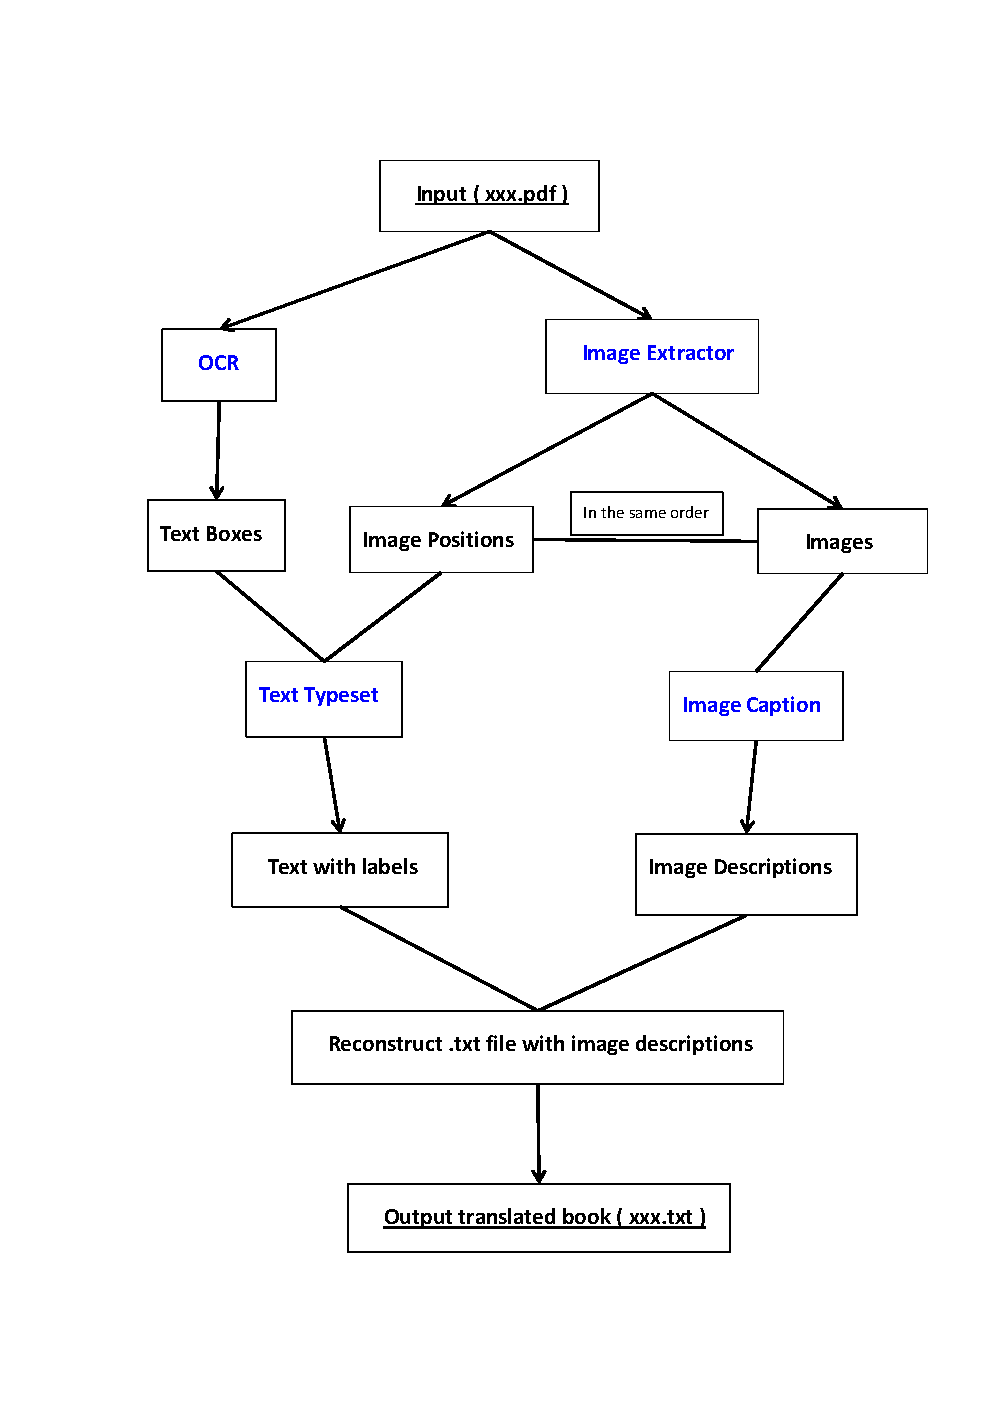
\includegraphics[width=0.8\linewidth]{figures/Overview.png}
    \caption{Pipeline}
    \label{fig:fig1}
\end{figure}

\end{document}